\section{Event Structure Semantics of DyNetKAT}
In this section, first, we introduce Normal DyNetKAT grammar.
Then we define different constructions on labeled event structures
which will be used to provide denotational semantics for Normal
DyNetKAT terms.

\subsection{Normal DyNetKAT}

Let $F = \s{f_1,...,f_n}$ be a set of field names with 
values in $V_i$, for $i \in \s{1,...,n}$.
We call complete test, denoted by $\alpha$
an expression $f_1 = v_1 \cdot ... \cdot f_n = v_n$ with $v_i \in V_i$ for $i \in \s{1,...,n}$.
We call complete assignment, denoted by $\pi$, and expression 
$f_1 \la v_1\cdot ... \cdot f_n \la v_n$ with $v_i \in V_i$ for 
$i \in \s{1,...,n}$.
We define the Normal DyNetKAT grammar as follows:
\begin{align*}
    F ::= & \alpha\cdot\pi                                                                           \\
    D ::= & \bot ~|~ F;D ~|~ x?F;D ~|~ x!F;D ~|~ D \parallel D ~|~ D \oplus D ~|~ \delta_{\mc{L}}(D) \\
          & \mc{L} = \s{c ~|~ c ::= x?F ~|~ x!F}
\end{align*}
In the following we use Normal DyNetKAT as a subset of DyNetKAT programs
to provide event structure semantics.

\subsection{Denotational Semantics of Normal DyNetKAT}

\begin{definition}
    Let $\mc{A}$ be an alphabet of letters of the form
    $\alpha \cdot \pi$,
    $x?F$, and $x!F$.
    We define the semantic map of Normal DyNetKAT terms
    $\sem{ \ }: D \ra \mathbb{E}$ where
    $\mathbb{E}$ is the set of all event structures with
    labels in $\mc{A}$ as follows:
    \begin{align*}
        \sem{\bot}      & = (\emptyset,\emptyset)                  \\
        \sem{\alpha; t} & = \alpha\sem{t}                        \\
        \sem{t_1 \oplus t_2}
                        & = \sem{t_1} + \sem{t_2}                  \\
        \sem{\delta_{\mc{L}}(t)}
                        & = \sem{t} \lceil (\mc{A} \setminus \mc{L}) \\
        \sem{t_1 \parallel t_2}
                        & = \sem{t_1} \times \sem{t_2}
    \end{align*}
    Where $\mc{L}$ is a subset of $\mc{A}$.
\end{definition}

\subsection{Examples}
In the following, we provide some examples to illustrate
how the prefix, sum, and product operators can be used to 
compose event structures.
For simplicity, here we use $a,b,c$ to denote DyNetKAT actions.

\begin{example}
    Let $a,b\in \mc{A}$ be some DyNetKAT actions and $a;b$ a
    normal DyNetKAT term.
    $\mr{E} = \sem{a;b}$ is an event structure
    $(E,\#,\vdash,L,l)$ where:
    \begin{align*}
        E  & = \s{(0,a),(1,0,b)}                       \\
        \# & = \emptyset                               \\
           & \e \vdash (0,a), \s{(0,a)} \vdash (1,0,b) \\
        L  & = \s{a,b}                                 \\
           & l((0,a)) = a, l((1,0,b)) = b              
    \end{align*}
    The following diagram shows configurations of $\mr{E}$:
    \begin{center}
        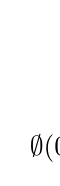
\begin{tikzpicture}[scale=0.8]
            \crd[right]{0}{0}{$\emptyset$}
            \crd[right]{0}{1}{$\s{(0,a)}$}
            \crd[right]{0}{2}{$\s{(0,a),(1,0,b)}$}
            \draw [ultra thick] (0,0) -- (0,1);
            \draw [ultra thick] (0,1) -- (0,2);
        \end{tikzpicture}
    \end{center}
\end{example}

\begin{example}
    Let $a,b\in \mc{A}$ be some DyNetKAT actions and $a\oplus b$ a
    normal DyNetKAT term.
    $\mr{E} = \sem{a\oplus b}$ is an event structure
    $(E,\#,\vdash,L,l)$ where:
    \begin{align*}
        E & = \s{(0,a),(1,b)}                \\
          & (0,a) \# (1,b)   \\
          & \e \vdash (0,a), \e \vdash (1,b) \\
        L & = \s{a,b}                        \\
          & l((0,a)) = a, l((1,b)) = b       
    \end{align*}
    The following diagram shows configurations of $\mr{E}$:
    \begin{center}
        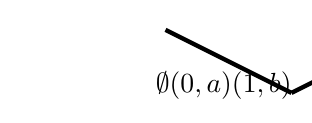
\begin{tikzpicture}[scale=0.8]
            \crd[above]{0}{0}{$\emptyset$}
            \crd[above]{-2}{1}{$\s{(0,a)}$}
            \crd[above]{2}{1}{$\s{(1,b)}$}
            \draw [ultra thick] (0,0) -- (-2,1);
            \draw [ultra thick] (0,0) -- (2,1);
        \end{tikzpicture}
    \end{center}
\end{example}


\begin{example}
    Let $a,b\in \mc{A}$ be some DyNetKAT actions and $a\parallel b$ a
    normal DyNetKAT term.
    $\mr{E} = \sem{a\parallel b}$ is an event structure
    $(E,\#,\vdash,L,l)$ where:
    \begin{align*}
        E  & = \s{(a,*),(*,b),(a,b)}                           \\
        \# & = \e                                              \\
           & \e \vdash (a,*), \e \vdash (*,b),\e \vdash (a,b)  \\
        L  & = \s{(a,*),(*,b),(a,b)}                           \\
           & l((a,*)) = (a,*), l((*,b)) = (*,b),l((a,b))=(a,b) 
    \end{align*}
    The following diagram shows configurations of $\mr{E}$:
    \begin{center}
        \begin{tikzpicture}[scale=0.8]
            \crd[above]{0}{0}{$\emptyset$}
            \crd[left]{-2}{1}{$\s{(a,*)}$}
            \crd[right]{2}{1}{$\s{(*,b)}$}
            \crd[above]{0}{2}{$\s{(a,*),(*,b)}$}
            \crd[above]{2}{3}{$\s{(a,b)}$}
            \draw [ultra thick] (0,0) -- (-2,1);
            \draw [ultra thick] (0,0) -- (2,1);
            \draw [ultra thick] (2,1) -- (0,2);
            \draw [ultra thick] (-2,1) -- (0,2);
            \draw [ultra thick] (0,0) -- (2,3);
        \end{tikzpicture}
    \end{center}
\end{example}